\documentclass[11pt,largemargins]{homework}
\usepackage{xeCJK}
\usepackage{amsthm}
\usepackage{amsmath}

\usepackage{tikz}
\usetikzlibrary{calc}
\usepackage{amsmath,amssymb}
\usepackage{tikz-cd}
\usetikzlibrary{fit}
\usetikzlibrary{arrows.meta}
\usepackage{enumitem}


\newcommand{\hwname}{蘇則宇}
\newcommand{\hwemail}{B11201005}
\newcommand{\hwtype}{Homework}
\newcommand{\hwnum}{10}
\newcommand{\hwclass}{Modern Algebra I}
\newcommand{\hwlecture}{}
\newcommand{\hwsection}{}

% This is just used to generate filler content. You don't need it in an actual
% homework!
\usepackage{lipsum}
\begin{document}
	\maketitle
	\question
	First check $L(M,N;P)$ is a $A-$mod. Let $f,g\in L(M,N;P)$ and $a\in A$, then $(a\cdot f+g):M\times N\rightarrow P$, $(a\cdot f+g)(x,y)=af(x,y)+g(x,y)$ is a $A-$bilinear map.
	\begin{enumerate}[label=(\alph*)]
		\item 
		For every $f\in L(M,N;P)$, exists a unique $A-$mod homomorphism $M\otimes_A N \xrightarrow{\tilde{f}} P$ s.t. $\tilde{f}(x\otimes y)=f(x,y)$. \\Conversely, any $\phi\in\text{Hom}_A(M\otimes N,P)$ defines a bilinear map $M\times N\rightarrow P$, a routine verification check that such relation is a $A-$mod isomorphism.
		\item 
		Will show an isomorphism:
		\begin{equation*}
			\text{Hom}(M\otimes N,P)\xrightarrow{\phi} \text{Hom}(M,\text{Hom}(N,P))
		\end{equation*}
		Let $f\in \text{Hom}(M\otimes N,P)$, then define $[\phi(f)(x)](y)=f(x\otimes y)\in P$. $A-$linear is trivial.\\
		Let $M\xrightarrow{g}\text{Hom}(N,P)$, $\bar{g}(x,y)=g(x)(y)\in P, x\in M,y\in N$ defines a $A-$bilinear map, hence exists a unique $A-$mod homomorphism\\ $M\otimes N\xrightarrow{\tilde{g}} P$ s.t. $\tilde{g}(x\otimes y)=\bar{g}(x,y)$.\\
		The existence shows onto, and the uniqueness shows one-to-one.
		\item Same as (b) since $N\otimes M\cong N\otimes M$.
		
		
		
	\end{enumerate}
	\question
	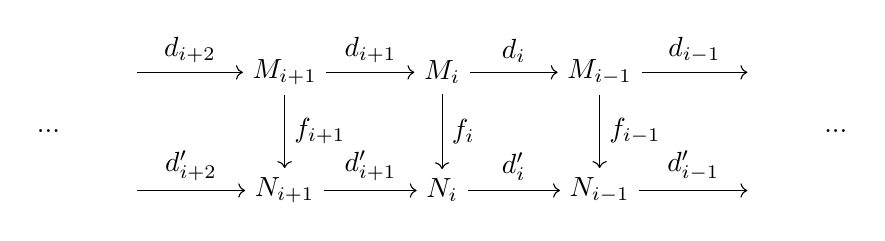
\begin{tikzpicture}
		\node(U1) at (2,0){};
		\node(D1) at (2,-1.5){};
		\node(U2) at (10,0){};
		\node(D2) at (10,-1.5){};
		\node(M3) at (4,0) {$M_{i+1}$};
		\node(M2) at (6,0) {$M_i$};
		\node(M1) at (8,0) {$M_{i-1}$};
		\node(N3) at (4,-1.5) {$N_{i+1}$};
		\node(N2) at (6,-1.5) {$N_i$};
		\node(N1) at (8,-1.5) {$N_{i-1}$};
		
		\draw[->] (M3)--(M2) node[midway,above]{$d_{i+1}$};
		\draw[->] (M2)--(M1) node[midway,above]{$d_{i}$};
		\draw[->] (N3)--(N2) node[midway,above]{$d^{\prime}_{i+1}$};
		\draw[->] (N2)--(N1) node[midway,above]{$d^{\prime}_{i}$};
		\draw[->] (U1)--(M3) node[midway,above]{$d_{i+2}$};
		\draw[->] (D1)--(N3) node[midway,above]{$d^{\prime}_{i+2}$};
		\draw[->] (M1)--(U2) node[midway,above]{$d_{i-1}$};
		\draw[->] (N1)--(D2) node[midway,above]{$d^{\prime}_{i-1}$};
		
		\draw[->] (M3)--(N3) node[midway,right]{$f_{i+1}$};
		\draw[->] (M2)--(N2) node[midway,right]{$f_i$};
		\draw[->] (M1)--(N1) node[midway,right]{$f_{i-1}$};
		
		\node() at (1,-0.75){$...$};
		\node() at (11,-0.75){$...$};
	\end{tikzpicture}
	\question
	Can see if the diagram commute, then $f_i$ maps ker$(d_i)$ to ker$(d^{\prime}_{i})$, and maps maps Im$(d_i)$ to Im$(d^{\prime}_{i})$ for all $i$.
\end{document}